%
\chapter{Il problema del monitoraggio}
Terminata la breve panoramica sugli impianti fotovoltaici, introduciamo il 
problema oggetto del presente lavoro di tesi: il monitoraggio degli 
impianti fotovoltaici.
%

%
\section{Obiettivi}
L'obiettivo di un sistema di monitoraggio, secondo \cite{dirks06}, consiste 
nella raccolta e nell'integrazione di tutti i dati \emph{rilevanti} dell'impianto 
fotovoltaico, al fine di determinare, nel tempo:
%
\begin{itemize}
\item lo \emph{stato operativo} dell'impianto stesso
\item l'efficienza globale dell'impianto
\item la quantit\`a di energia prodotta
\item lo stato di salute e il degrado prestazionale dei singoli componenti
\end{itemize}
%

%
Una pi\`u articolata definizione delle finalit\`a di un sistema di monitoraggio
\`e presentata in \cite{kolodenny08}. L'approccio consiste nella 
individuazione di tre \emph{classi} di utenti a seconda del loro ruolo, i.e.
a seconda del tipo di informazioni, relative all'impianto monitorato,
cui essi sono interessati:
%
\begin{itemize}
\item \emph{ricercatore}, i.e. \emph{una persona che analizza tutti i dati disponibili 
alla ricerca di possibili relazioni}; i ricercatori sono, generalmente, interessati 
ad avere quanti pi\`u dati possibili, ad un livello di dettaglio quanto pi\`u elevato
possibile
%
\item \emph{proprietario}, i.e. il soggetto responsabile dell'impianto; le informazioni
cui i soggetti responsabili sono, tipicamente, maggiormente interessati sono \Item{i}
quanta energia il suo sistema sta producendo e \Item{ii} se la quantit\`a di energia 
prodotta \`e comparabile con le stime pre-investimento
%
\item \emph{tecnico}, i.e. il soggetto manutentore dell'impianto; i manutentori sono
interessati ad essere notificati rapidamente di tutti i possibili sintomi di malfunzionamento 
e/o di ogni comportamento non regolare dell'impianto, al fine di diagnosticarne le cause
\end{itemize}
%

%
\section{Identificazione delle grandezze rilevanti}
Alla base di ogni sistema di monitoraggio vi \`e un \emph{outdoor data acquisition system} 
(DAS), ovvero un sistema di acquisizione dati costituito da un insieme di sensori 
e da una infrastruttura di comunicazione che consente di rilevare il valore di 
determinate \emph{variabili di campo}. 
%% la produzione e` un processo continuo
Intuitivamente, la scelta delle variabili di campo da monitorare dipende fortemente dalla 
classe di utenti che costituiranno gli \emph{end-user} del sistema di monitoraggio.
%
Ad esempio, per fornire ai proprietari informazioni circa il rendimento dei loro impianti 
\`e sicuramente necessario monitorare, mediante apposita sensoristica, la potenza scambiata 
con la rete di distribuzione. La sola conoscenza della potenza scambiata, invece, potrebbe 
non essere sufficiente ai manutentori.
%
Supponiamo, ad esempio, che si rilevi una potenza prodotta inferiore al 75\% della potenza di picco
dell'impianto (la maggior parte degli impianti, causa mismatch di corrente, ombreggiamenti e 
altre condizizioni indesiderabili, mostra, normalmente, una resa media inferiore al 20-25\% rispetto 
alla potenza di picco\cite{roman06}) e che si desideri individuare le cause di tale degrado 
di performance.
%
In linea teorica, un calo di potenza potrebbe essere dovuto sia a un malfunzionamento 
di un componente, sia a un momentaneo annuvolamento. Per cui, informazioni utili per 
l'identificazione delle cause del problema sono anche le correnti delle singole stringhe e le 
condizioni metereologiche del sito ove l'impianto \`e installato.
%
Come fatto notare in \cite{kolodenny08}, \emph{pi\`u l'insieme delle informazioni rilevanti 
\`e completo, pi\`u rapida e affidabile sar\`a la procedura di diagnostica di ogni 
malfunzionamento del sistema}.
%% parlare del predictive monitoring?
%

%
In generale, un insieme di \emph{grandezze rilevanti} adatto a qualunque esigenza 
di monitoraggio, \`e ricavabile da una analisi delle soluzioni proposte in letteratura
\cite{xiaoli11}, \cite{dirks06}, \cite{kolodenny06}, \cite{aristizabal06}: %%\cite{benghanem98}:
%
\begin{itemize}
\item tensioni, correnti e potenze in punti specifici dell'impianto
\item temperatura ambientale
\item temperatura dei dispositivi
\item irraggiamento
\item velocit\`a e direzione del vento
\end{itemize}
%
%% ---> alcune variabili possono essere stimate
%
\section{Acquisizione dati}
Il monitoraggio delle grandezze rilevanti, richiede l'installazione sul campo e 
l'interfacciamento di sensori di vario tipo (sensori di corrente, di irraggiamento, etc.)
%

%
%% i sensori utilizzati sono spesso disegnati appositamente per il fotovoltaico (kolodenny08)
Per l'acquisizione dei dati generati dai sensori, i sistemi di monitoraggio proposti in 
letteratura adottano le soluzioni pi\`u disparate:
%
\begin{itemize}
\item in \cite{roman06}, la comunicazione con i sensori di campo avviene sfruttando  
      le stesse \emph{power line} dell'impianto e, quindi, senza alcuna necessit\`a di 
      cablaggi aggiuntivi; i sensori vengono interrogati periodicamente da un PLC
\item in \cite{xiaoli11} viene proposto un approccio basato sull'implementazione di una 
      \emph{wireless sensor network} (WSN): ogni sensore \`e dotato di un transponder 
      ZigBee\cite{zigbee} che gli permette di interfacciarsi con una \emph{base station},
      il cui compito \`e quello di raccogliere e integrare i dati di tutti i sensori;
      come la soluzione precedente, anche in questo caso non vi \`e necessit\`a di 
      cablaggi aggiuntivi
\item in \cite{guozhen09} vengono affrontate alcune problematiche legate 
      all'implementazione di sistemi SCADA per il monitoraggio di impianti fotovoltaici
\end{itemize}
%
La scelta del sistema di acquisizione da utilizzare \`e anch'essa frutto delle esigenze 
di monitoraggio. 
%
Sistemi basati su bus industriali gestiti da PLC o SCADA sono in grado di 
offrire delle garanzie di consegna dei dati di tipo \emph{real time}; 
%
soluzioni di questo tipo potrebbero essere adottate nei casi in cui, ad esempio, 
si abbia la necessit\`a di tracciare, con estrema precisione, l'andamento nel tempo 
di grandezze caratterizzate da alta \emph{variabilit\`a}, p.es. l'irraggiamento.
D'altro canto si tratta di sistemi che richiedono cablaggi dedicati e, nel complesso, 
non sono di immediata installazione e configurazione.
%

%
Una soluzione basata su WSN, d'altra parte, \`e pi\`u economica e semplice da 
installare e configurare, a fronte di una ridottissima capacit\`a a far fronte a 
esigenze di monitoraggio tempo critiche.
%
\section{Presentazione dei dati}
Oltre all'acquisizione dei dati di campo, un sistema di monitoraggio deve essere in grado
di processare, trasformare e pubblicare i dati raccolti al fine di renderli accessibili e 
di rappresentarli in un formato adatto alle finalit\`a dell'attivit\`a di monitoraggio.
%

%
Come per le precedenti questioni, anche la scelta del tipo di rappresentazioni da produrre 
e delle piattaforme software da utilizzare per la loro produzione dipende fortemente 
dallo scopo del sistema di monitoraggio.
%
Ad esempio, una rappresentazione utile per fornire ai proprietari degli impianti 
informazioni circa l'andamento della produzione \`e riportata in figura 
\ref{esempiopotenza}: si tratta del grafico che rappresenta l'andamento della 
potenza prodotta nell'arco di 24 ore.
%
\begin{figure}[!hpb]
\centering
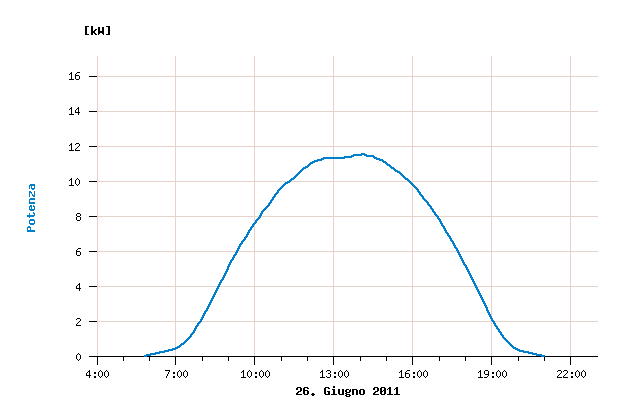
\includegraphics[width=350pt]{img/fv-trend-potenza.jpg}
\caption{Trend di potenza generata nell'arco di 24 ore}
\label{esempiopotenza}
\end{figure}
%

%
Ovviamente, non si tratta dell'unico tipo di grafico o rappresentazione derivabile dai 
dati di campo. Potrebbero essere prodotti, a scopo diagnostico, dei grafici che mettano a 
confronto l'andamento dell'irraggiamento con quello della potenza. Oppure l'andamento 
della dell'irraggiamento con quello delle correnti di stringa.
%
Altre possibili rappresentazioni verranno trattate nel capitolo\ref{sec:datapresentation}.
%

%
Per quanto riguarda le piattaforme utilizzate, \`e interessante notare come la
maggior parte delle soluzioni gi\`a citate \cite{kolodenny06}, \cite{xiaoli11}, 
\cite{dirks06} pubblichi e rappresenti i dati mediante una \emph{web application}.


%% quale tecnologia utilizzare?
%% anche la rappresentazione dipende dal tipo di sistema implementato
%% ad esempio, la presentazione deve poter facilitare il compito al tecnico
%% indicando subito eventuali parametri fuori norma

%%\section{Un sistema di monitoraggio large scale per applicazioni business}
%% lista dei desiderata per un sistema di monitoraggio
